%---------------------------------------------------------
%	PRESENTATION BODY SLIDES
%---------------------------------------------------------
\section{ЭДМ исследования} % Note all sections and subsections are automatically placed in your table of contents

\begin{frame}
 \frametitle{Научная группа по исследованию ЭДМ}
 \begin{enumerate}
 	\item Научный руководитель Сеничев Ю.В. профессор, доктор ф.-м. наук;
 	\item Аксентьев А.Е. кандидат ф.-м. наук "Метод замороженного спина  для поиска электрического дипольного момента дейтрона в накопительном кольце.";
 	\item Мельников А.А. кандидат ф.-м. наук "Исследование спин-орбитального движения и управления поляризацией в накопительном кольце для поиска электрического дипольного момента лёгких ядер."
 	\item Колокольчиков С.Д. аспирант "Исследование динамики поляризованного пучка в ускорительном комплексе NICA-Nuclotron в приложении к изучению электрического дипольного момента легких ядер."
 	\item Паламарчук П.И. бакалавр 4 курс "Исследование ЭДМ в кольцевых установках."
 \end{enumerate}

\end{frame}

\begin{frame}
 \frametitle{Электричкеский дипольный момент}

	\begin{figure}
		\centering
		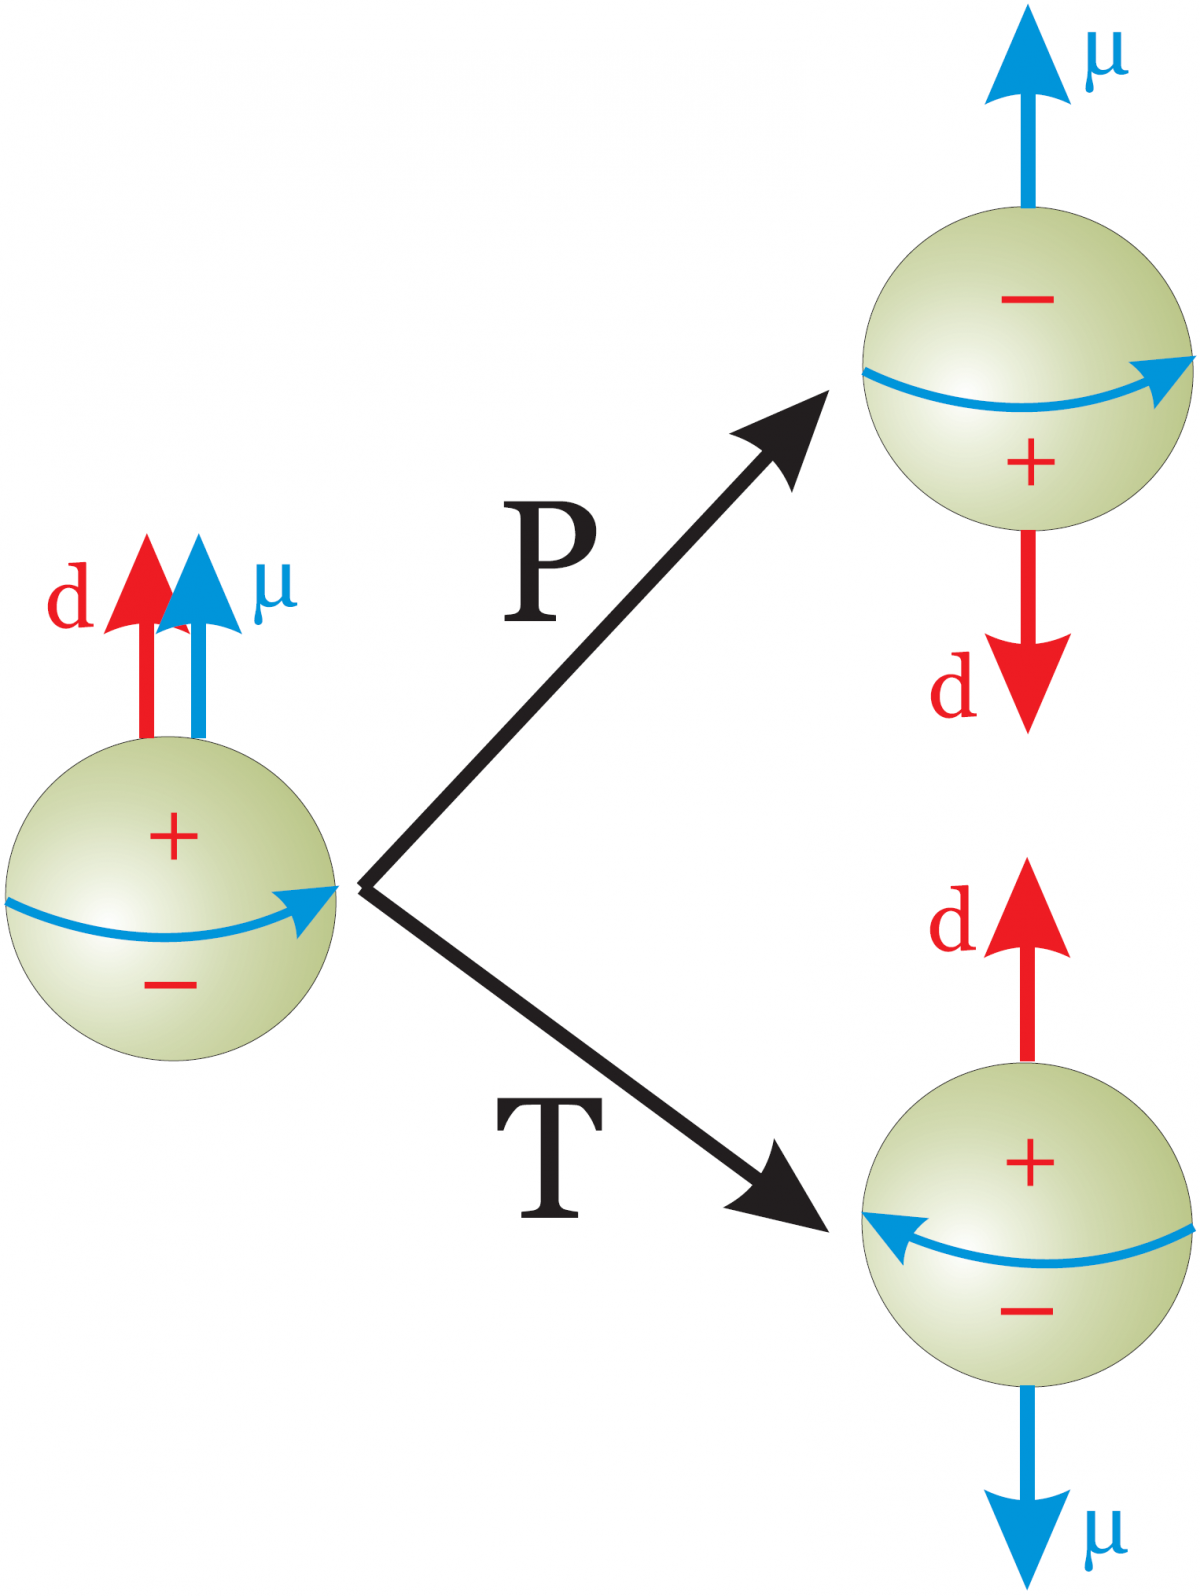
\includegraphics[width=0.3\linewidth]{images/edm_cp}
	\end{figure}

	
\end{frame}

\begin{frame}
\frametitle{Эволюция спина}
	\textbf{Теорема Эренфеста}: средние значения квантовых операторов эволюционируют во времени в соответствии с классическими уравнениями движения, если гамильтониан системы не зависит явно от времени. Это важный мостик между квантовой и классической физикой, показывающий, как классические законы вытекают из квантовых принципов.
\newline \newline
\textbf{Уравнение Т-БМТ} эволюции спина -- прецессия спина от магнитного дипольного момента (МДМ) и электрического дипольного момента (ЭДМ).
\begin{equation} \label{eq:T-BMT}
	\frac{{d \vec{S}}}{d t} =\vec{S} \times\left(\vec{\Omega}_{\textrm{MDM}}+\vec{\Omega}_{\textrm{EDM}}\right)
\end{equation}

\end{frame}

\begin{frame}
	\frametitle{География ЭДМ}
	\begin{figure}
		\centering
		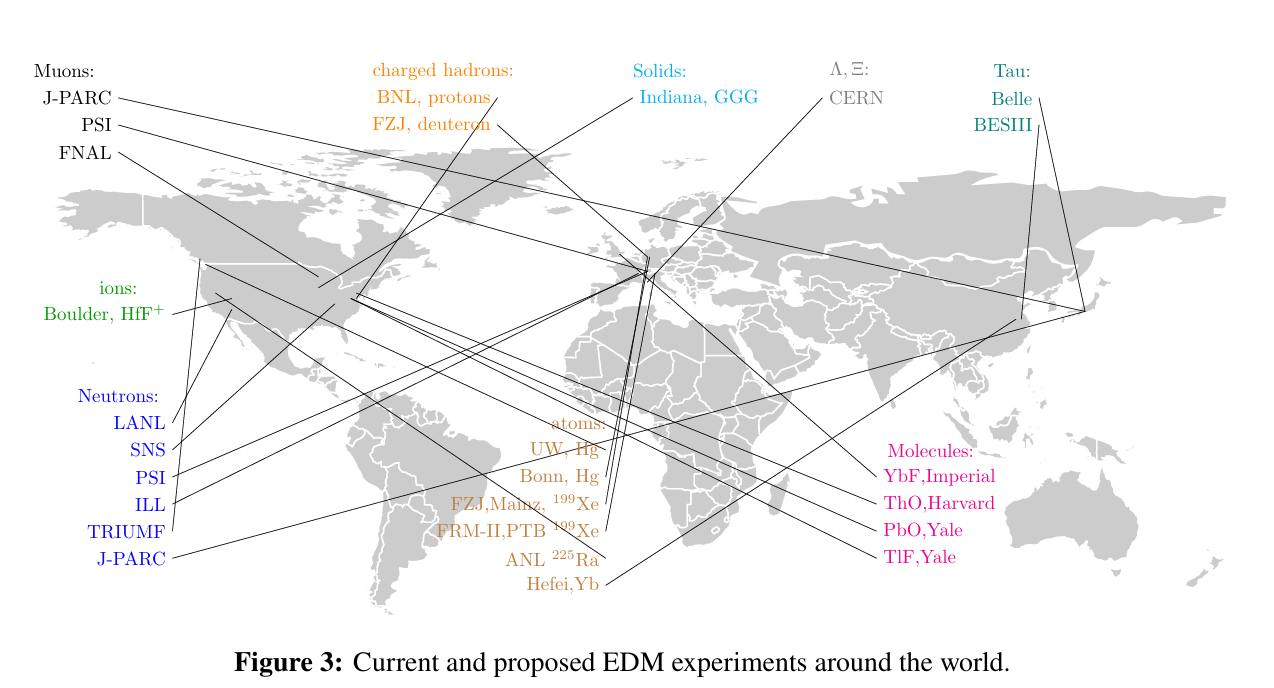
\includegraphics[width=0.8\linewidth]{images/edm_geo}
	\end{figure}
	
	
\end{frame}
%------------------------------------------------